\documentclass[twocolumn,prd,superscriptaddress,amsfonts,amssymb,amsmath,preprintnumbers]{revtex4-1}
\usepackage{epsfig}
\usepackage{graphics}
\usepackage{graphicx}
\usepackage{bm}
\usepackage[dvipsnames]{xcolor}
\usepackage{bm}
\usepackage{times}
\usepackage{xspace}
\usepackage[varg]{txfonts}
\usepackage[normalem]{ulem} % To get strikethrough (\sout)
\usepackage[colorlinks]{hyperref}
\usepackage[caption=false]{subfig}
\usepackage{booktabs}
\usepackage{url}
\usepackage{float}
\usepackage[bottom]{footmisc}
\usepackage{lineno}
\linenumbers




\definecolor{LinkColor}{rgb}{0.75, 0, 0}
\definecolor{CiteColor}{rgb}{0, 0.5, 0.5}
\definecolor{UrlColor}{rgb}{0, 0, 0.75}
\hypersetup{linkcolor=LinkColor}
\hypersetup{citecolor=CiteColor}
\hypersetup{urlcolor=UrlColor}
\usepackage{perpage}
\MakePerPage{footnote}

\newcommand{\paperone}{Paper~I\xspace}
\newcommand{\abhi}[1]{\textcolor{red}{[\textit{AG: #1}]}}
\newcommand{\rb}[1]{\textcolor{blue}{[\textit{RB: #1}]}}

\newcommand{\h}{\mathpzc{h}}
\newcommand{\Hhat}{\hat{\mathpzc{H}}}
\newcommand{\B}{\mathpzc{B}}
\newcommand{\hlm}{\mathpzc{h}_{\ell m}}
\newcommand{\xilm}{\xi_{\ell m}}
\newcommand{\Ylm}{{Y}^{-2}_{\ell m}}
\newcommand{\Y}{{Y}^{-2}}
\newcommand{\hc}{h_\times}
\newcommand{\hp}{h_+}
\newcommand{\Fc}{F_\times}
\newcommand{\Fp}{F_+}
\newcommand{\Mf}{M_f}
\newcommand{\cA}{\mathpzc{A}}
\newcommand{\lm}{_{\ell m}}
\newcommand{\deff}{d_\mathrm{eff}}
\newcommand{\rmi}{\mathrm{i}}
\newcommand{\blambda}{\bm{\lambda}}
\newcommand{\btheta}{\bm{\theta}}
\newcommand{\bxi}{\bm{\xi}}
\newcommand{\bxigr}{\bm{\xi}_{\text{GR}}}
\newcommand{\bxingr}{\bm{\xi}_{\text{nGR}}}
\newcommand{\bzeta}{\bm{\zeta}}
\newcommand{\bs}[1]{\bm{\vec{s}_{#1}}}
\newcommand{\Mo}{M_{\odot}}
\newcommand{\FFe}{\mathrm{FF}_\mathrm{eff}}
\newcommand{\FF}{\mathrm{FF}}
\newcommand{\e}{\mathrm{e}}
\newcommand{\rhoopt}{\rho_\mathrm{opt}}
\newcommand{\rhosubopt}{\rho_\mathrm{subopt}}
\newcommand{\fqnm}{f}
\newcommand{\sigmaqnm}{\sigma}
\newcommand{\n}{\mathbf{n}}
\newcommand*{\skymapscale}{0.5}
\newcommand*{\paramestscale}{0.455}
\newcommand{\df}[1]{\delta f_{\text{#1}}}
\newcommand{\dtau}[1]{\delta \tau_{\text{#1}}}
\newcommand{\fngr}[1]{f_{\text{#1}}}
\newcommand{\taungr}[1]{\tau_{\text{#1}}}
\newcommand{\fgr}[1]{f ^{\text{GR}}_{\text{#1}}}
\newcommand{\taugr}[1]{\tau ^{\text{GR}}_{\text{#1}}}
\newcommand{\pSEOB}{\texttt{pSEOBNR}}
\newcommand{\SEOB}{\texttt{SEOBNR}}

\begin{document}

\title{Black hole symphony orchestra: Spectroscopy using gravitational wave signals from binary black hole coalescences}

\author{Abhirup Ghosh}
\affiliation{Max Planck Institute for Gravitational Physics (Albert Einstein Institute), D-14476 Potsdam-Golm, Germany}
\author{Richard Brito}
\affiliation{Dipartimento di Fisica, ``Sapienza" Universit`a di Roma $\&$ Sezione INFN Roma1, Piazzale Aldo Moro 5, 00185, Roma, Italy}
\author{Alessandra Buonanno}
\affiliation{Max Planck Institute for Gravitational Physics (Albert Einstein Institute), D-14476 Potsdam-Golm, Germany}

\date{\today}


%%%%%%%%%%%%%%%%%%%%%%%
\begin{abstract}
The no-hair conjecture in General Relativity states that the properties of a Kerr black hole (BH) are completely described by its mass and spin angular momentum. As a consequence, the complex quasi-normal-mode (QNM) frequencies of a binary black hole (BBH) ringdown can be uniquely determined by the mass and spin of the remnant object. Conversely, measurement of the QNM frequencies could be a independent test of the no-hair conjecture. This paper outlines a test of the no-hair conjecture by measuring the complex QNM frequencies of a BBH ringdown within the framework of, for the first time, a spinning inspiral-merger-ringdown waveform model, thereby using the entire signal power and removing dependency on the predicted or estimated start time of the proposed ringdown. We further demonstrate the robustness of the test against modified gravitational wave (GW) signals with a ringdown different from what GR predicts for Kerr BHs. The method was used to analyse the properties of the merger remnants for the events observed by LIGO-Virgo in the first half of their third observing run (O3a) in the latest LIGO-Virgo publication. In this paper, for the first time, we analyse the GW events from the first and second LIGO-Virgo observing runs and provide joint constraints with published results from O3a. We also analyse two events from the O3a list of events that were not considered for the initial analysis. Finally, the joint measurements of the fractional deviations in the frequency, $\df{220} = XX \pm$ and $\dtau{220} = YY \pm$ are the strongest constraints yet using this method. %Finally, we also present a investigation into possible systematic effects due to an incomplete understanding of the interferometric noise around the GW event on the results of this test.
\end{abstract}
%%%%%%%%%%%%%%%%%%%%%%%

\maketitle


\section{Introduction}\label{sec:intro}

The LIGO Scientific Collaboration~\citep{lsc} and the Virgo Collaborations~\citep{Virgo} recently announced their catalogue of gravitational wave (GW) observations~\citep{GWTC-2} from the first half of their third observing run (O3a)~\citep{O3reference}. Combined with the confirmed observations from the first and second observing runs~\citep{abbott2019gwtc}, the Advanced LIGO detectors at Hanford, Washington and Livingston, Louisiana~\citep{aasi2015characterization}, and the Advanced Virgo detector in Cascina, Italy~\citep{acernese2014advanced} have now detected more than $50$ GW events from the merger of compact objects like neutron stars and/or black holes (BHs), collectively called compact binary coalescences (CBCs). Alongside independent claims of detections~\citep{nitz20191,nitz20202,2019PhRvD.100b3007Z,2020PhRvD.101h3030V,Venumadhav_2020}, this has firmly established the field of GW astronomy, five years on from the first ever direct detection of GWs on Earth, on September 14, 2015~\citep{abbott2016observation}.
\par
Observation of GWs have had significant astrophysical and cosmological implications~\citep{LSC_2016astroph,gw170817_mma,gw170817_joint,gw170817_hubble}. It has also allowed us to make statements in fundamental physics. Specifically, LIGO-Virgo's observations have allowed us to test predictions of Einstein's theory of General Relativity (GR)~\citep[GR]{}, in previously unexplored regimes of highly relativistic, strong-field regimes of gravity~\citep{LSC_2016grtests,GW170817_TGR,gwtc1_tgr}. In GR, a CBC involving two BHs (a binary black hole (BBH) system) is described in three distinct phases: an early \textit{inspiral}, where the two compact objects spiral in and \textit{plunge} due to a back-reaction of gravitational-wave-emission, a \textit{merger} marked by the formation of an apparent horizon~\citep{NRpaper}, and a late-time \textit{ringdown}, where the newly formed remnant object settles down to a stable Kerr state through the emission of an exponentially damped quasi-normal-mode (QNM) spectrum of gravitational radiation~\citep{vishu,earlyqnmpapers}.  
\par
The LIGO-Virgo collaborations have also released a companion paper detailing their latest results of tests of GR using events from the catalogues GWTC-2 CITE and GWTC-1 CITE. The results include tests of GW generation and source dynamics, where bounds are placed on parametrised deviations in the Post-Newtonian coefficients describing the early inspiral~\citep{earlydevelopmentpapers}, and phenomenological coefficients describing the intermediate (plunge) and merger regimes of coalescence~\citep{TIGERmethodspapers}, tests of GW propagation, which assume a generalised dispersion relation and place upper bounds on the Compton wavelength and consequently, the mass of the graviton~\citep{gw170104,samajdar2017projected} and tests of the polarisation of gravitational radiation using a multi-gravitational-wave-detector network~\citep{gw170814,isi2017probing}. The paper also checks for consistency between different portions of the signal using estimates of predicted mass and spin of the remnant object~\citep{Ghosh:2016xx,Ghosh:2017gfp,LSC_2016grtests}, and consistency of the residuals with interferometric noise~\citep{Ghonge:2020suv,gwtc1_tgr}. None of these tests report any departure from the predictions of GR.
\par
The LIGO-Virgo O3a testing GR paper also details results on tests of BH ringdown and nature of the remnant object, which is an active field of research at the moment. The no-hair conjecture in GR~\citep{} states that an (electrically neutral) astrophysical BH is completely described by two observables: mass and spin angular momentum. One consequence of the no-hair conjecture is that the (complex) QNM frequencies of gravitational radiation emitted by a perturbed isolated BH is uniquely determined by its mass and spin angular momentum. Hence a test of the no-hair conjecture would involve checking for consistency between estimates of mass and spin of the remnant object across multiple QNM frequencies. An inconsistency would either indicate a non-BH nature of the remnant object, or an incompleteness of GR as the underlying theory of gravity. The consistency between the post-merger signal and the least damped QNM was first demonstrated in ~\citep{LSC_2016grtests} for GW150914, and later extended to include overtones in~\citep{Brito:2018rfr,Giesler:2019uxc,Isi:2019aib,Bhagwat:2019dtm,Forteza:2020hbw}. Consistency of the late-time signal with a single QNM is a test of the ringdown of a BBH coalescence, but not necessarily a test of the no-hair conjecture, which requires the measurement of (at least) two QNMs (BH spectroscopy), and checking for consistency between them. Recent work in that direction include~\citep{Carullo:2018gah,Carullo:2019flw,Bhagwat:2019bwv}. The nature of the remnant object has also been explored through tests of BH thermodynamics, like the Hawking's area theorem~\citep{Cabero:2017avf} or through search for echos in the post-merger signal~\citep{Nielsen:2018lkf,Tsang:2019zra,Lo:2018sep,Abedi:2018npz,Abedi:2020sgg,Testa:2018bzd}. None of these tests have found evidence for non-BH nature of the remnant object (as described in GR) in LIGO-Virgo BBH observations.
\par
Most of the tests mentioned above focus on analysing the post-merger or late-time ringdown signal in isolation. Second generation ground-based interferometric detectors like Advanced LIGO and Virgo are most sensitive to stellar-mass BH binaries that merge near the minima of their sensitivity band ($\sim 100$Hz). As a consequence, the remnant object \textit{rings down} in shot-noise dominated higher frequencies, leaving very little signal-to-noise ratio (SNR) in the post-merger signal. The ringdown start time is not a clearly defined quantity and has been explored in detail in~\citep{Bhagwat:2017tkm}. In other works~\citep{Carullo:2018gah,Carullo:2019flw}, it has been left as a free parameter to be estimated directly from the data. Uncertainties in estimates of the ringdown start-time, as well as an overall lack of SNR in the post-merger signal, given typical sensitivities of ground-based detectors result in significant statistical uncertainties in the measurement of the QNM frequencies.
\par
An independent approach to BH spectroscopy, based on a full-signal analysis, was outlined in~\citep{Brito:2018rfr} (henceforth referred to as \paperone). Unlike methods that focus on the post-merger signal, it describes a framework in which a complete inspiral-merger-ringdown (IMR) waveform model is used to measure the complex QNM frequencies. This allows access to the full SNR of the signal, reducing measurement uncertainties. Moreover, the definition of the ringdown start time is built into the model and does not need to be either left as an additional free parameter or fixed using alternate definitions. While \paperone presented the method in the context of a non-spinning waveform model, we extend the analysis to the case with BHs spins in the current paper. \abhi{mention other improvements between EOBNRv2 and EOBNv4} All astrophysical BHs are expected to be spinning, and ignoring effects of spin have been shown to introduce systematic biases in the measurement of the source properties CITE \cite{paper_showing_systematics_from_ignoring_spin}.
\par
The rest of this paper is organized as follows. Section~\ref{sec:model} describes our parametrised IMR waveform model. In section~\ref{sec:method}, we define our testing GR framework in which we use that model to measure the complex QNM frequencies within a Bayesian formalism. Then in section~\ref{sec:results}, we demonstrate our method on real GW events, as well as simulated signals. Finally we provide a summary of our results and discuss future developments in section~\ref{sec:discussion}.

\section{Method}

A GW signal from the (quasi-circular) coalescence of two BHs is completely described in GR by a fixed set of $15$ parameters, $\bxigr$. These can be grouped into the \emph{intrinsic} parameters: the masses, $m_1, m_2$ and spins, $\bs1, \bs2$ of the initial binary and a reference time and phase $t_c, \phi_c$ respectively; and the \emph{extrinsic} parameters: the sky position of the binary ($\alpha$, $\delta$), the luminosity distance, $d_L$, and its orientation described through the inclination of the binary $\iota$ and its polarisation $\psi$. If the spins of the individual BHs are assumed to be aligned with the orbital angular momentum of the binary, then GW signal has a reduced dimensionality of $11$ parameters. The aligned-spin components are defined as: $a_{iz} = s_{iz}/m_i$, where $i=1,2$ for the two BHs.

\subsection{Waveform Model}\label{sec:model}

As in \paperone, we use an IMR waveform model developed within the EOB formalism. However, in this work we extend the results of \paperone by using a waveform model for spinning, non-precessing BBHs. Namely we use as our baseline model the aligned-spin multipolar waveform developed in Ref.~\citep{Cotesta:2018fcv}. In addition to being calibrated to NR simulations, this model also uses information from BH perturbation theory for the merger and ringdown phases. Therefore this waveform model provides a very accurate and faithful semi-analytic description of the inspiral, merger and ringdown phases. Henceforth we will denote this model by $\SEOB$ for short.


In the observer's frame, the GW polarizations can be written as 
%
\begin{equation}
h_+(\iota,\varphi;t ) - i h_\times(\iota,\varphi;t) = \sum_{\ell, m} {}_{-\!2}Y_{\ell m}(\iota,\varphi)\, h_{\ell m}(t)\,,
\end{equation}
%
where $\varphi$ is the azimuthal direction to the observer, ${}_{-\!2}Y_{\ell m}(\theta,\phi)$ are the $-2$ spin-weighted spherical harmonics. The $\SEOB$ model we employ includes the $(\ell, |m|)=(2,2),(2,1)$, $(3,3)$, $(4,4)$, and $(5,5)$ modes~\cite{Cotesta:2018fcv}. For each $(\ell, m)$, the inspiral-(plunge-)merger-ringdown $\SEOB$ waveform is schematically given by
%
\begin{equation}
h_{\ell m}(t) = h_{\ell m}^\mathrm{insp-plunge}\, \theta(t_\mathrm{match}^{\ell m} - t) + h_{\ell m}^\mathrm{merger-RD}\,\theta(t-t_\mathrm{match}^{\ell m})\,,
\end{equation}
where $\theta(t)$ is the Heaviside step function, $h_{\ell m}^\mathrm{insp-plunge}$ represents the inspiral-plunge part of the waveform, whereas $h_{\ell m}^\mathrm{merger-RD}$ denotes the merger-ringdown phase.   
The merger-ringdown $\SEOB$ modes read~\citep{Bohe:2016gbl,Cotesta:2018fcv}
%
\begin{equation}
\label{RD}
h_{\ell m}^{\textrm{merger-RD}}(t) = \nu \ \tilde{A}_{\ell m}(t)\ e^{i \tilde{\phi}_{\ell m}(t)} \ e^{-i \sigma_{\ell m 0}(t-t_{\textrm{match}}^{\ell m})},
\end{equation}
%
where $\nu$ is the symmetric mass ratio of the binary and $\sigma_{\ell m0} = 2\pi f_{\ell m 0} -i/\tau_{\ell m 0}$ denotes the complex frequency of the fundamental QNMs of the remnant BH. We denote the oscillation frequencies by $f_{\ell m  0}\equiv \Re(\sigma_{\ell m0})/(2\pi)$ and the decay times by $\tau_{\ell m 0}\equiv -1/\Im(\sigma_{\ell m0}) $. 
The functions $\tilde{A}_{\ell m}(t)$ and $\tilde{\phi}_{\ell m}(t)$ are given by~\cite{Bohe:2016gbl,Cotesta:2018fcv}:
%
\begin{equation}
\label{eq:ansatz_amp}
\tilde{A}_{\ell m}(t) = c_{1,c}^{\ell m} \tanh[c_{1,f}^{\ell m}\ (t-t_{\textrm{match}}^{\ell m}) \ +\ c_{2,f}^{\ell m}] \ + \ c_{2,c}^{\ell m},
\end{equation}
%
\begin{equation}
\label{eq:ansatz_phase}
\tilde{\phi}_{\ell m}(t) = \phi_{\textrm{match}}^{\ell m} - d_{1,c}^{\ell m} \log\left[\frac{1+d_{2,f}^{\ell m} e^{-d_{1,f}^{\ell m}(t-t_{\textrm{match}}^{\ell m})}}{1+d_{2,f}^{\ell m}}\right],
\end{equation}
%
where $ \phi_{\textrm{match}}^{\ell m}$ is the phase of the inspiral-plunge mode $(\ell, m)$ computed at $t = t_{\textrm{match}}^{\ell m}$. The coefficients $d_{1,c}^{\ell m}$ and $c_{i,c}^{\ell m}$ with $i = 1,2$
are fixed by imposing that the functions $\tilde{A}_{\ell m}(t)$ and $\tilde{\phi}_{\ell m}(t)$ are of class $C^1$ at $t = t_{\textrm{match}}^{\ell m}$, when matching the merger-ringdown waveform to the inspiral-plunge $\SEOB$ waveform $h_{\ell m}^\mathrm{inspiral-plunge}(t)$. This allows to write the coefficients $c_{i,c}^{\ell m}$ as~\cite{Cotesta:2018fcv}:
% in terms of $c_{1,f}^{\ell   m},\ c_{2,f}^{\ell m},\ \sigma^\textrm{R}_{\ell m},\ |h_{\ell    m}^{\textrm{insp-plunge}}(t_{\textrm{match}}^{\ell  m})|,\ \partial_t|h_{\ell    m}^{\textrm{insp-plunge}}(t_{\textrm{match}}^{\ell m})|$ as
\begin{align} 
c_{1,c}^{\ell m} &= \frac{1}{c_{1,f}^{\ell
    m} \nu} \big[ \partial_t|h_{\ell
    m}^{\textrm{insp-plunge}}(t_{\textrm{match}}^{\ell m})| \nonumber \\
    &- \sigma^\textrm{R}_{\ell m} |h_{\ell
    m}^{\textrm{insp-plunge}}(t_{\textrm{match}}^{\ell
    m})|\big] \cosh^2{(c_{2,f}^{\ell m})}, \\
c_{2,c}^{\ell m} &= -\frac{ |h_{\ell
    m}^{\textrm{insp-plunge}}(t_{\textrm{match}}^{\ell
    m})|}{\nu} + \frac{1}{c_{1,f}^{\ell
    m} \nu} \big[ \partial_t|h_{\ell
    m}^{\textrm{insp-plunge}}(t_{\textrm{match}}^{\ell m})|  \nonumber \\
    &- \sigma^\textrm{R}_{\ell m} |h_{\ell
    m}^{\textrm{insp-plunge}}(t_{\textrm{match}}^{\ell
    m})|\big] \cosh{(c_{2,f}^{\ell m})}\sinh{(c_{2,f}^{\ell m})}, \\ \nonumber   
\end{align}
and $d_{1,c}^{\ell m}$ as
\begin{align}    
d_{1,c}^{\ell m} &= \left[\omega_{\ell m}^{\textrm{insp-plunge}}(t_{\textrm{match}}^{\ell m}) -  \sigma^\textrm{I}_{\ell
      m}\right]\frac{1+ d_{2,f}^{\ell m}}{d_{1,f}^{\ell m}d_{2,f}^{\ell m}}\,,
\end{align}
%
where we denoted $\sigma_{\ell m}^\textrm{R} \equiv \Im (\sigma_{\ell m0}) < 0$ and  $\sigma_{\ell m}^\textrm{I} \equiv -\Re (\sigma_{\ell m0})$, and $\omega_{\ell m}^{\textrm{insp-plunge}}(t)$ is the frequency of the inspiral-plunge EOB mode. The coefficients $c_{i,f}^{\ell m}$ and $d_{i,f}^{\ell m}$ are obtained through fits to NR and 
Teukolsky-equation--based waveforms and can be found in Appendix C of Ref.~\cite{Cotesta:2018fcv}.

In the $\SEOB$ model constructed in Ref.~\cite{Cotesta:2018fcv}, the complex frequencies $\sigma_{\ell m 0}$  are expressed in terms of the final BH mass and spin~\cite{Berti:2005ys,Berti:2009kk}, and the latter are related to the BBH's component masses and spins through NR--fitting-formulas obtained in GR~\cite{Taracchini:2013rva,Hofmann:2016yih}. Here instead, in the spirit of what was done in \paperone, we promote the QNM (complex) frequencies to be free parameters of the model, while keeping the inspiral-plunge modes $h_{\ell m}^\mathrm{inspiral-plunge}(t)$ fixed to their GR values. Henceforth called $\pSEOB$, this model uses a parameterised version of the $\SEOB$ model where the frequency and the damping time of the ${\ell m 0}$ mode, i.e, $(f_{\ell m 0}, \tau _{\ell m 0})$ is defined through fractional deviations, ($(\delta f_{\ell m 0},\delta \tau_{\ell m 0})$), from the corresponding GR values, i.e., the predictions of the QNM frequencies obtained using the fits~\cite{Taracchini:2013rva,Hofmann:2016yih}:

\begin{eqnarray}
f_{\ell m 0} &:=& f_{\ell m 0}^{\text{GR}} (1 + \delta f_{\ell m 0})\label{eq:nongr_freqs_a} \\ 
\tau _{\ell m 0} &:=& \tau _{\ell m 0}^{\text{GR}} (1 + \delta \tau_{\ell m 0}) \label{eq:nongr_freqs_b}
\end{eqnarray}
The GR quantities $( f_{\ell m 0}^{GR},\tau_{\ell m 0}^{GR})$ are constructed using the same NR--fitting--formula prescriptiion described above. We note that when leaving $\sigma_{\ell m}$ to vary freely, the functions $\tilde{A}_{\ell m}(t)$ and $\tilde{\phi}_{\ell m}(t)$ will in general also differ from the GR prediction, since those functions depend on the QNM complex frequencies, as can be seen from the expressions for $c_{i,c}^{\ell m}$ and $d_{1,c}^{\ell m}$.


\subsection{Bayesian PE}\label{sec:method}

The parametrised model, $\pSEOB$, described above introduces an additional set of non-GR parameters, $\bxingr = (\delta f_{\ell m 0},\delta \tau_{\ell m 0})$, corresponding to each $(\ell,m)$ QNM present in the GR waveform model $\SEOB$. One then proceeds to use the Bayes theorem to obtain the \emph{posterior} probability distribution on $\blambda = \{\bxigr, \bxingr\}$, given a hypothesis $\mathcal{H}$:

\begin{equation}
P(\blambda | d, \mathcal{H}) = \frac{P(\blambda | \mathcal{H}) \, \mathcal{L}(d | \blambda, \mathcal{H})}{P(d|\mathcal{H})},
\label{eq:Bayes_theorem}
\end{equation}
where $P(\blambda | \mathcal{H})$ is the \emph{prior} probability distribution, and $\mathcal{L}(d | \blambda, \mathcal{H})$ is called the \emph{likelihood} function. The denominator is a normalization constant $P(d|\mathcal{H}) := \int P(\blambda | \mathcal{H}) \, \mathcal{L}(d | \blambda, \mathcal{H}) \, d\blambda$, called the marginal likelihood, or the \emph{evidence} of the hypothesis $\mathcal{H}$. In this case, our hypothesis $\mathcal{H}$ is that the data contains a GW signal that is described by the $\pSEOB$ waveform model $h(\blambda)$  and stationary Gaussian noise described by a power spectral density (PSD) $S_n(f)$. The likelihood function can consequently be defined as:

\begin{equation}
\mathcal{L}(d | \blambda, \mathcal{H}) \propto \exp\big[-\frac{1}{2} \langle d - h(\blambda) \, | \, d -h(\blambda) \rangle \big],
\label{eq:likelihood}\end{equation}
where $\langle . | . \rangle$ is the following noise-weighted inner product:
\begin{equation}
\langle A | B \rangle := \int_{f_\mathrm{low}} ^{f_\mathrm{high}} df \frac{\tilde{A}^*(f)\tilde{B}(f) + \tilde{A}(f)\tilde{B}^*(f)}{S_n(f)}.
\label{eq:nwip}
\end{equation}
$\tilde{A}(f)$ denotes the Fourier transform of $A(t)$ and a $^*$ denotes complex conjugation. The limits of integration ${f_\mathrm{low}}$ and ${f_\mathrm{high}}$ define the bandwidth of the sensitivity of the GW detector. We usually assume ${f_\mathrm{high}}$ to be the Nyquist frequency whereas${f_\mathrm{low}}$ is dictated by the response of the gravitational detector to low-frequency seismic noise. Owing to the large dimensionality of the parameter set $\blambda$, the posterior distribution $P(\blambda | d, \mathcal{H})$ in equation~(\ref{eq:Bayes_theorem}) is computed by stochastically sampling the parameter space using techniques such as Markov-Chain Monte-Carlo~\cite{xxx} or Nested Sampling~\cite{xxx}. For this paper, we use the lalinferencemcmc~\cite{xx} and bilby codes CITE that provide an implementation of the parallely tempered MCMC and Nested Sampling algorithms respectively, for computing the posterior distributions. 

Given the full-dimensional posterior probability density function $P(\blambda | d, \mathcal{H})$, we can marginalise over the \emph{nuisance} parameters, to obtain the marginalised posterior probability density function over the QNM parameters $\bxingr$:

\begin{equation}
P(\bxingr | d, \mathcal{H})= \int P(\blambda | d, \mathcal{H}) d\bxigr
\end{equation}

For most of the results discussed in this paper, we would restrict ourselves to the $(\ell m) = (2,2)$ and/or $(3,3)$ modes. In those cases we would assume $\bxingr = \{\df{220},\dtau{220}\}$ and/or  $ \{\df{330},\dtau{330}\}$, and all the other $(\ell m)$ modes to be fixed at their GR predictions, i.e., $\delta f_{\ell m 0} = \delta \tau_{\ell m 0} = 0$. This is because, for most of the high-mass events we find most appropriate for this test, the LIGO-Virgo observations are consistent with nearly-equal-mass face-on/off BH binaries for which power in the subdominant modes is not enough to attempt to measure more than one, or at most QNM frequencies simultaneously. 

Throughout our analysis, we assume uniform priors on our non-GR QNM parameters, $(\delta f_{\ell m 0},\delta \tau_{\ell m 0})$. However, since the priors on $( f_{\ell m 0}^{GR},\tau_{\ell m 0}^{GR})$ are derived through NR--fits, from the corresponding priors on the initial masses and spins, this leads to a non-trivial prior on the final reconstructed frequency and damping time, $( f_{\ell m 0},\tau_{\ell m 0})$. Also, given the definition of the damping time in Sec.~\ref{sec:model}, we realise $\delta \tau_{\ell m 0} = -1$ leads to the imaginary part of the frequency going to infinity. We avoid this by restricting the minimum of the prior on $\delta \tau_{\ell m 0}$ to be greater than $-1$.

\iffalse
\subsection{Priors}

Throughout our analysis we assume a completely prior uniform in the component masses $m_1, m_2$. Our prior on the spins are uniform in the magnitude between (0,1) and isotropic in spin orientation, but finally restricted to the component parallel to the orbital angular momentum of the binary. The prior on the distance varies as $d_L^2$ giving more weightage to binaries farther out. For the rest of the parameters we use standard priors as defined in the documentation (CITE Vietch et al. 2015 LALInference paper). For our non-GR ringdown parameters, we assume uniform priors. This of course leads to a non-trivial prior on the reconstructed frequency and damping time, because of the prior on $( f_{\ell m 0}^{GR},\tau_{\ell m 0}^{GR})$, which itself depend on the prior on the initial masses and spins through NR fits \abhi{perhaps figure on priors on QNM quantities}. For $d\tau = -1$, we encounter a singularity (the imaginary part of the frequency goes to infinity), which we avoid by restricting the minimum of the prior on $d\tau$ to be greater than $-1$.
\fi

\section{Results}\label{sec:results}

\subsection{Simulations using GR signals in Gaussian Noise}\label{ssec:gr_signal}

First, we demonstrate our method on GW signals from BBH systems that are well described by GR. We inject simulated GW signals modellng inspiral, merger and ringdown of BBHs into coloured Gaussian noise with PSDs expected at design sensitivities of Advanced LIGO-Virgo CITE. In particular we choose parameters similar to two specific GW events, GW150914 CITE and GW190521 CITE. The details of the injections are provided in Table~\ref{tab:injection_values}. These two systems are representative data points for the kind of systems this test is most suitable for: high-mass events which are loud enough that the SNR pre- and post-merger return reliable parameter estimation results. To avoid possible systematic biases in our parameter estimation results due to error in modelling, we use the GR version of the same waveform, $\SEOB$ (without allowing for deviations in the QNM parameters) to simulate our GW signal. And to avoid systematic biases due to noise, we use an averaged (zero-noise) realisation of the noise. A detailed study on noise systematics for one of the GW events is presented in Appendix~\ref{sec:noise_systematics}. As in the case of the actual detections, we consider a two-detector advanced LIGO network at Hanford and Livingston, having identical PSDs. The distance to the two simulated events is rescaled such that the SNR in the detector network is same as the actual event, i.e, 24 (14) for GW150914 (GW190521). Since (almost) equal-mass binaries like GW150914 and GW190521 observed at moderately high SNRs are not expected to have a loud ringdown signal, we restrict ourselves to estimating the frequency and damping time of the $(\ell m) = (2,2)$, i.e., $\{\df{220},\dtau{220}\}$, while fixing the other QNM frequencies to their GR values. 

We find, as one might expect, that the posterior distribution on the parameters describing fractional deviations in the frequency and damping time are consistent with zero (left panels of Fig.~\ref{fig:simulated_signal_GR}). One can then convert these fractional quantities into absolute quantities using the relations given in Eqs.~\ref{eq:nongr_freqs_a} and ~\ref{eq:nongr_freqs_b}, and construct posterior distributions on these effective quantities, $(\fngr{220}, \taungr{220})$ (right panels of Fig.~\ref{fig:simulated_signal_GR}). In each of these cases, recovered posterior are consistent with the GR predictions (black solid lines).

\iffalse
%%%%%%%%%%%%%%%%%%%%%%%%%%%%%%%%%%%%%%%%%%%%%%%%%%%%%%%%%%%%%%%
% Table for Injections
%%%%%%%%%%%%%%%%%%%%%%%%%%%%%%%%%%%%%%%%%%%%%%%%%%%%%%%%%%%%%%%
\begin{table}[h!]
\begin{center}
\begin{tabular}{ |c|c|c|c|c|c| }
 \hline
 Event & $m_1 (\Mo)$ &  $m_1 (\Mo)$ & $a_{1z}$ & $a_{2z}$ & SNR \\ 
 \hline
 GW150914 & 38.53 & 33.40 & 0.0035 & -0.0440 & 25 \\ \label{tab:injection_values}
 GW190521 & 152.20 & 120.41 & 0.0230 & -0.3864 & 14 \\ 
 \hline
\end{tabular}
\caption{Details of the injection parameters, chosen to be similar to the actual GW events}
\label{tab:injection_values}
\end{center}
\end{table}
%%%%%%%%%%%%%%%%%%%%%%%%%%%%%%%%%%%%%%%%%%%%%%%%%%%%%%%%%%%%%%%
%%%%%%%%%%%%%%%%%%%%%%%%%%%%%%%%%%%%%%%%%%%%%%%%%%%%%%%%%%%%%%%
\fi

%%%%%%%%%%%%%%%%%%%%%%%%%%%%%%%%%%%%%%%%%%%%%%%%%%%%%%%%%%%%%%%
% Table for Injections
%%%%%%%%%%%%%%%%%%%%%%%%%%%%%%%%%%%%%%%%%%%%%%%%%%%%%%%%%%%%%%%
\begin{table}[h!]
\begin{center}
\begin{tabular}{ |c|c|c|c|c|c| }
 \hline
 Event & $m_{1,d} (\Mo)$ &  $m_{2,d} (\Mo)$ & $a_{1z}$ & $a_{2z}$ & SNR \\ 
 \hline
 GW150914 & 39 & 31 & 0.0 & 0.0 & 25 \\
 GW190521 & 150 & 120 & 0.02 & -0.39 & 14 \\ 
 SXS:BBH:0166 & 72 & 12  & 0.0 & 0.0 & 75 \\
 \hline
\end{tabular}
\caption{Details of the injection parameters, chosen to be similar to the actual GW events. $(m_{1,d},m_{2,d})$ are the detector-frame masses of the primary and secondary BHs respectively.}
\label{tab:injection_values}
\end{center}
\end{table}
%%%%%%%%%%%%%%%%%%%%%%%%%%%%%%%%%%%%%%%%%%%%%%%%%%%%%%%%%%%%%%%
%%%%%%%%%%%%%%%%%%%%%%%%%%%%%%%%%%%%%%%%%%%%%%%%%%%%%%%%%%%%%%%

%%%%%%%%%%%%%%%%%%%%%%%%%%%%%%%%%%%%%%%%%%%%%%%%%%%%%%%%%%%%%%%
% Simulated siganl: GR
%%%%%%%%%%%%%%%%%%%%%%%%%%%%%%%%%%%%%%%%%%%%%%%%%%%%%%%%%%%%%%%
\begin{figure}[h!]
	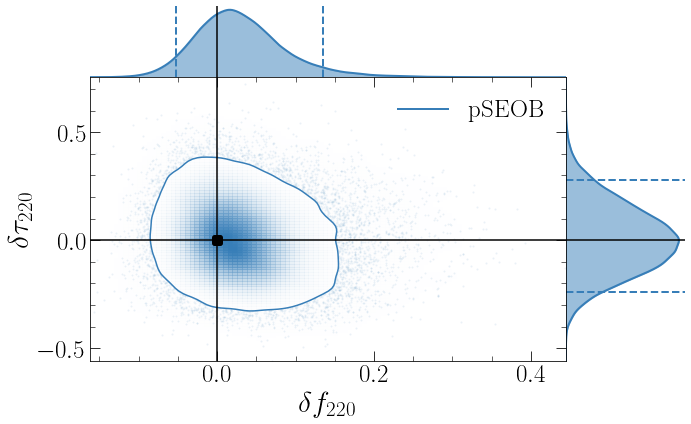
\includegraphics[width=0.25\textwidth]{figures/GW150914_simulated_signal_0p0_deltaf220_deltatau220.png}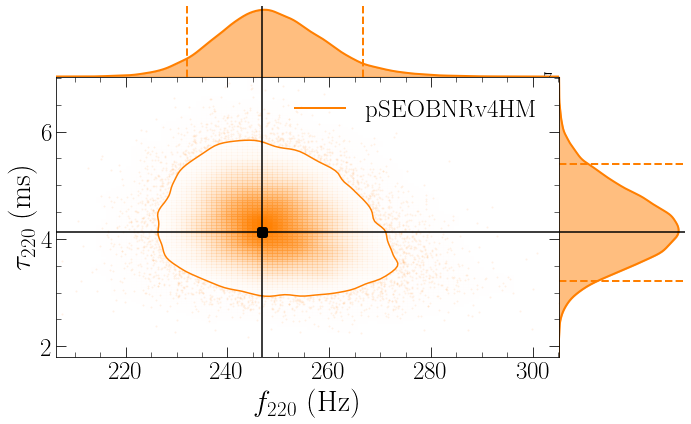
\includegraphics[width=0.25\textwidth]{figures/GW150914_simulated_signal_0p0_f220_tau220.png}	
	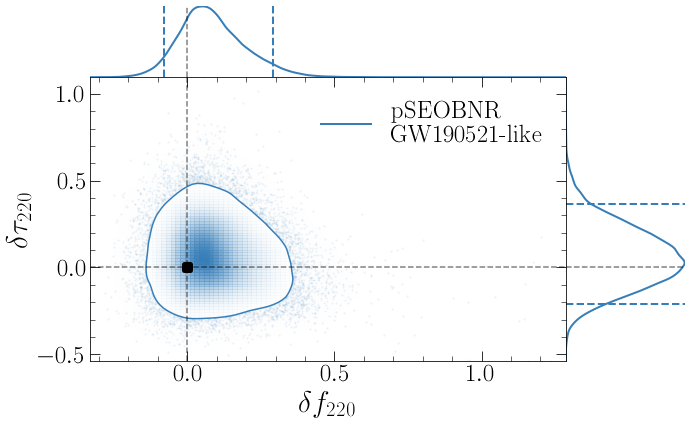
\includegraphics[width=0.25\textwidth]{figures/GW190521_simulated_signal_0p0_deltaf220_deltatau220.png}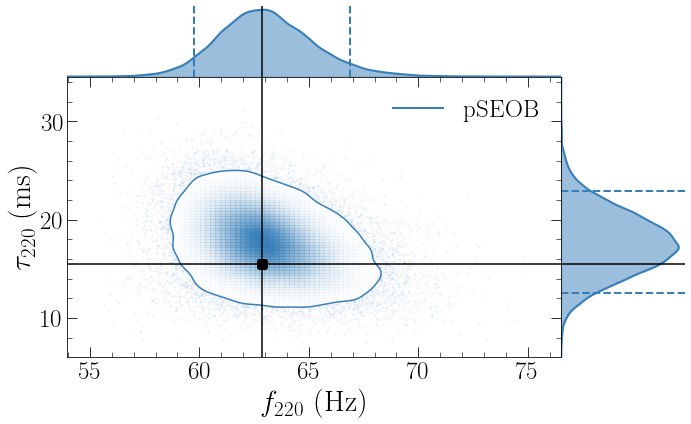
\includegraphics[width=0.25\textwidth]{figures/GW190521_simulated_signal_0p0_f220_tau220.png}		
	\caption{\textcolor{red}{FINAL RESULT} Posterior probability distribution on the fractional deviations in the frequency and damping time of the $(2,2)$ QNM, $\{\df{220},\dtau{220}\}$ (left panels) and the reconstructed quantities, $(\fngr{220}, \taungr{220})$ (right panels) for GR injections with initial parameters similar to GW150914 (top panels) and GW190521 (bottom panels) (Table~\ref{tab:injection_values}). The 2D contour marks the 90\% credible region, while the dashed lines on the 1D marginalised distributions mark the 90\% credible levels. The black vertical and horizontal lines mark the injection values.}
	\label{fig:simulated_signal_GR}
\end{figure}
%%%%%%%%%%%%%%%%%%%%%%%%%%%%%%%%%%%%%%%%%%%%%%%%%%%%%%%%%%%%%%%
%%%%%%%%%%%%%%%%%%%%%%%%%%%%%%%%%%%%%%%%%%%%%%%%%%%%%%%%%%%%%%%

\subsection{Simulations using modified GR signals in Gaussian noise}

To demonstrate the robustness of the method in detecting possible deviations of the underlying GW signal from predictions of GR, we inject simulated GW signals which are identical to the corresponding GR prediction upto merger, and differ in their post-merger description. We again choose systems with initial-binary-parameters similar to GW150914 and GW190521, but we attach a phenomenological post-merger signal described by deviation parameters $\df{220} = \dtau{220} = 0.5$ \abhi{deviations=0.1 runs are ongoing and almost done}. In other words, we assume that the frequency and damping time of our non-GR signal is 1.5 times the corresponding GR prediction, although the pre-merger signal is identical to GR (Fig.\ref{fig:nongr_waveform}). We also avoid waveform and noise systematic biases by choosing a configuration identical to the simulations described in Sec.\ref{ssec:gr_signal}. The posterior probability distributions on $(\df{220}, \dtau{220})$ or equivalently $(\fngr{220}, \taungr{220})$ (Fig.~\ref{simulated_signal_nonGR}) are consistent with the corresponding the values of the injection parameters, indicated by the black solid lines. 

We additionally investigate the effects of erroneously assuming that an underlying modified GR signal can be well-described using GR. We do this by estimating the parameters of our modified GR signals using the GR waveform model $\SEOB$ instead of the parametrised $\pSEOB$. In such cases, we run the risk of biased parameter estimates due to an incomplete understanding of the underlying signal. The resulting posterior probability distributions are shown in the right panels of Fig.~\ref{simulated_signal_nonGR} by the pink (GW150914) and grey (GW190521) curves. The results are interesting and distinctly different for the two events. For the GW150914-like modified GR signal, the measurements of $(\fgr{220}, \taugr{220})$ (Fig.~\ref{simulated_signal_nonGR} top right panel) are consistent with the $(\fgr{220}, \taugr{220})$ measurements for a signal with no deviations (Fig.~\ref{simulated_signal_GR} top right panel). In other words, if the actual signal had deviations as large as the 50 \% of the GR prediction, the analysis with $\SEOB$ would likely have reported \emph{no} deviation from the GR prediction. However in the case of the GW190521-like modified GR signal, a simple GR analysis of the modified GR signal would have yielded measurements distinctly different from either of the two parametrised estimates: with and without deviations. The fact that the GW190521-like signal has a much lower SNR than GW150914 might be a possible reason for the the measurement of the final quantities to be more susceptible to noise. A more detailed comparison of the other parameters, like the masses and spins, between an $pSEOB$ and an $SEOB$ measurement of a modified GR signal is shown in the appendix (Fig.~\ref{fig:gr_ngr_comparison}).

%%%%%%%%%%%%%%%%%%%%%%%%%%%%%%%%%%%%%%%%%%%%%%%%%%%%%%%%%%%%%%%
%%%%%%%%%%%%%%%%%%%%%%%%%%%%%%%%%%%%%%%%%%%%%%%%%%%%%%%%%%%%%%%
\begin{figure}
	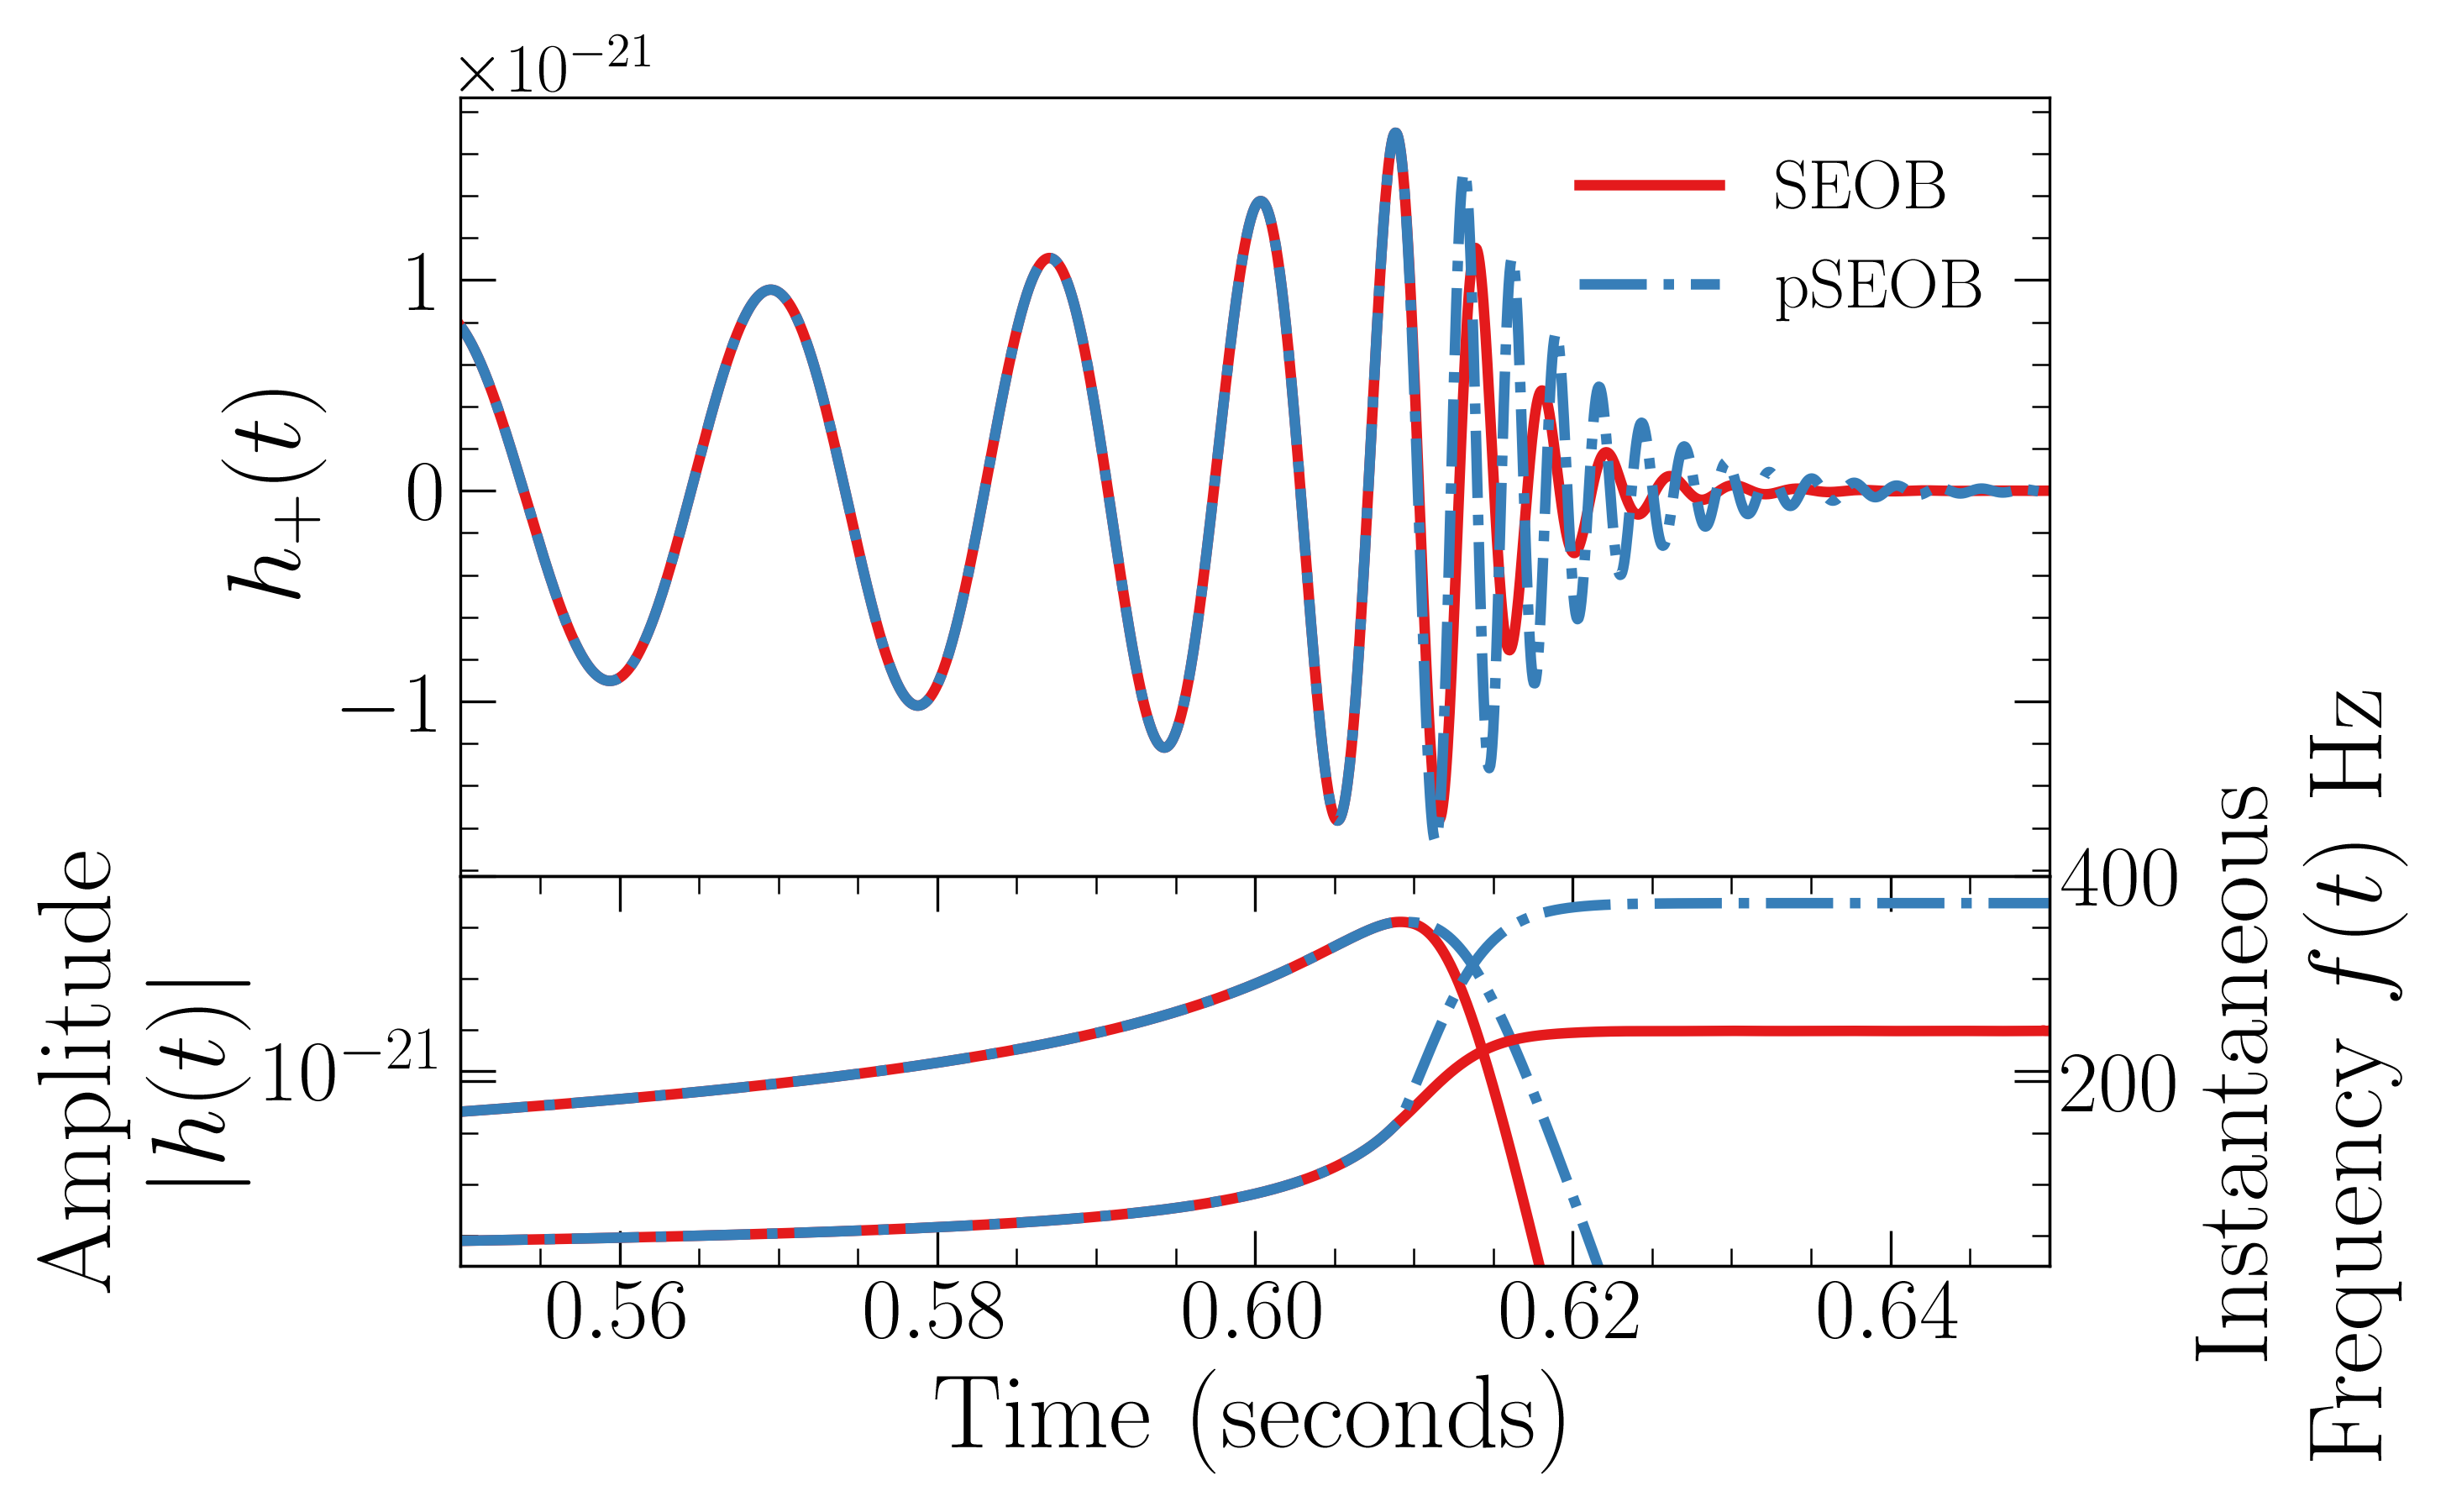
\includegraphics[width=0.5\textwidth]{figures/modGR_waveforms_amplitudephase.png}
	\caption{\textcolor{red}{FINAL RESULT} Top panel: The `+'--polarisation of the gravitational waveform $h_+(t)$ from a GW150914-like event where the post-merger is described by GR (solid orange lines), i.e., $\df{220} = \dtau{220} = 0$, and where the merger-ringdown is modified (dashed grey lines), i.e., $\df{220} = \dtau{220} = 0.5$. Bottom panel: Comparison of the evolution of the amplitude (left) and phase (right) for the GR and modified GR signal.}
	\label{fig:nongr_waveform}
\end{figure}
%%%%%%%%%%%%%%%%%%%%%%%%%%%%%%%%%%%%%%%%%%%%%%%%%%%%%%%%%%%%%%%
%%%%%%%%%%%%%%%%%%%%%%%%%%%%%%%%%%%%%%%%%%%%%%%%%%%%%%%%%%%%%%%

%%%%%%%%%%%%%%%%%%%%%%%%%%%%%%%%%%%%%%%%%%%%%%%%%%%%%%%%%%%%%%%
% Simulated siganl: non-GR
%%%%%%%%%%%%%%%%%%%%%%%%%%%%%%%%%%%%%%%%%%%%%%%%%%%%%%%%%%%%%%%
\begin{figure}[h!]
	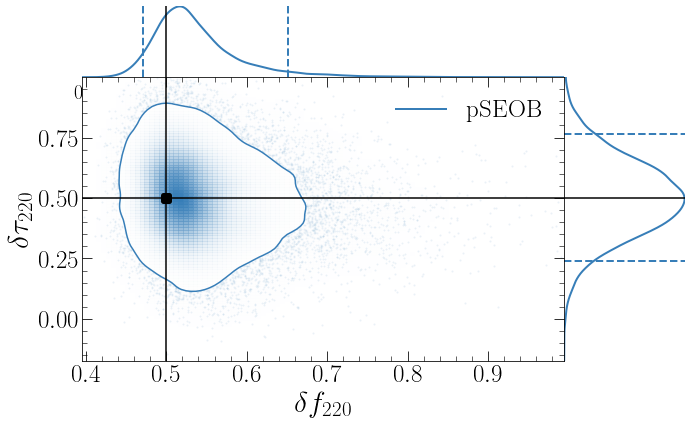
\includegraphics[width=0.25\textwidth]{figures/GW150914_simulated_signal_0p5_deltaf220_deltatau220.png}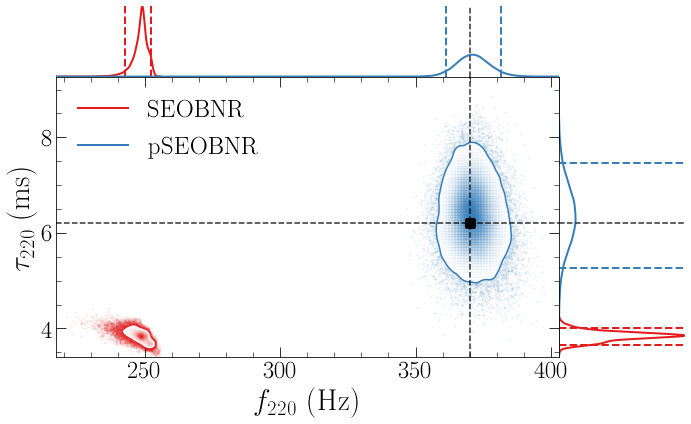
\includegraphics[width=0.25\textwidth]{figures/GW150914_simulated_signal_0p5_gr_ngr_fngrtaungr.png}	
	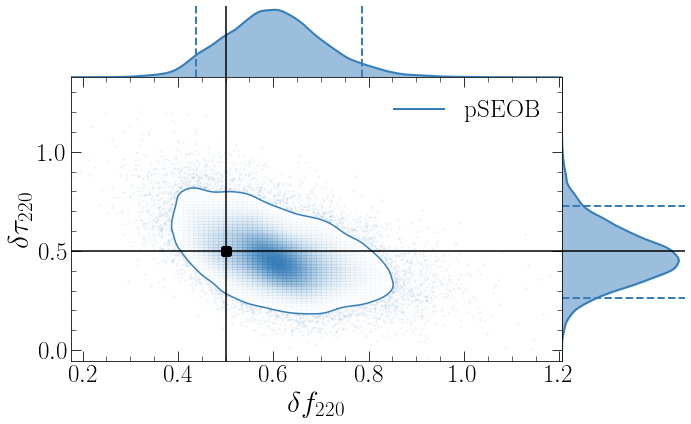
\includegraphics[width=0.25\textwidth]{figures/GW190521_simulated_signal_0p5_deltaf220_deltatau220.png}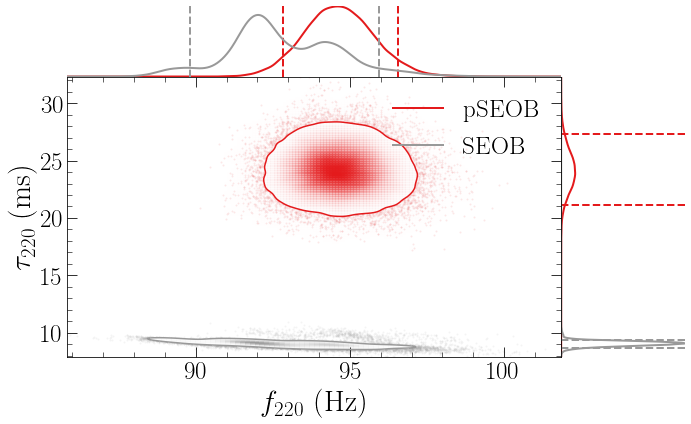
\includegraphics[width=0.25\textwidth]{figures/GW190521_simulated_signal_0p5_gr_ngr_fngrtaungr.png}
	\caption{\textcolor{red}{FINAL RESULT} Posterior probability distribution on the fractional deviations in the frequency and damping time of the $(2,2)$ QNM, $\{\df{220},\dtau{220}\}$ (left panels) and the reconstructed quantities, $(\fngr{220}, \taungr{220})$ (right panels) for modGR injections with initial parameters similar to GW150914 (top panels) and GW190521 (bottom panels) (Table~\ref{tab:injection_values}). The underlying signal has a deviation, $\df{220} = \dtau{220} = XX$. The 2D contour marks the 90\% credible region, while the dashed lines on the 1D marginalised distributions mark the 90\% credible levels. The black vertical and horizontal lines mark the injection values. In the right panels, we additionally show measurements using a GR ($SEOB$) waveform, for GW150914 (grey) and GW190521 (pink), The measurements are visibly biased.}
	\label{fig:simulated_signal_nonGR}
\end{figure}
%%%%%%%%%%%%%%%%%%%%%%%%%%%%%%%%%%%%%%%%%%%%%%%%%%%%%%%%%%%%%%%
%%%%%%%%%%%%%%%%%%%%%%%%%%%%%%%%%%%%%%%%%%%%%%%%%%%%%%%%%%%%%%%

\subsection{Test of the No hair theorem}\label{ssec:nohairtheorem}

Finally, we provide a simple demonstration of a test of the no-hair theorem using our model. As described in the introduction, any test of the no-hair theorem of BHs would need to involve independent measurements of (at least) two different QNMs. We use a simulated GW signal from the SXS catalog CITE corresponding a non-spinning BBH with a mass-ratio $q=6$ (SXS:BBH:0166), rescaled to a total mass of $M=84 \Mo$ (Table~\ref{tab:injection_values}). We choose an asymmetric system to increase the SNR in the higher modes. We also rescale the distance and orientation of the binary such that the total SNR of the signal in a network of three detectors, LIGO Hanford, Livingston and Virgo, is 75. Based on the LIGO-Virgo observations during O3a, such asymmetric and loud signals are no longer just a theoretical prediction but quite plausible at design sensitivities. Using this signal, we attempt to measure the QNM frequencies $(2,\pm 2)$ and $(3,\pm 3)$ modes together (Fig.~\ref{fig:nohair_sxs}). The SNR in other sub-dominant modes is too less for us to estimate them reliably.

The fractional deviations in the estimates of the damping time and frequency of either mode is expected to be consistent with 0, as we indeed find in the left panel of Fig.~\ref{fig:nohair_sxs}. Consequently we find that the reconstructed quantities $(\fngr{220}, \taungr{220})$ and $(\fngr{330}, \taungr{330})$  are also consistent with the corresponding predictions for a BBH merger in GR. As a consequence, the information from these two independent measures correspond to a unique remnant object, which is completely described by its mass and spin angular momentum \abhi{have the mf-af plot as well as a third panel to show consistency}. For most of the events observed so far, the power in the $(3,\pm 3)$ has not been sufficient to measure it along with the $(2,\pm 2)$, or in fact, in its place. However, it might also be possible to combine information from multiple observation, as is likely over the coming few years of GW astronomy with the LIGO-Virgo detectors, to obtain meaningful constraints on the $(3,\pm 3)$ and other sub-dominant QNMs.

%%%%%%%%%%%%%%%%%%%%%%%%%%%%%%%%%%%%%%%%%%%%%%%%%%%%%%%%%%%%%%%

%%%%%%%%%%%%%%%%%%%%%%%%%%%%%%%%%%%%%%%%%%%%%%%%%%%%%%%%%%%%%%%
\begin{figure}
	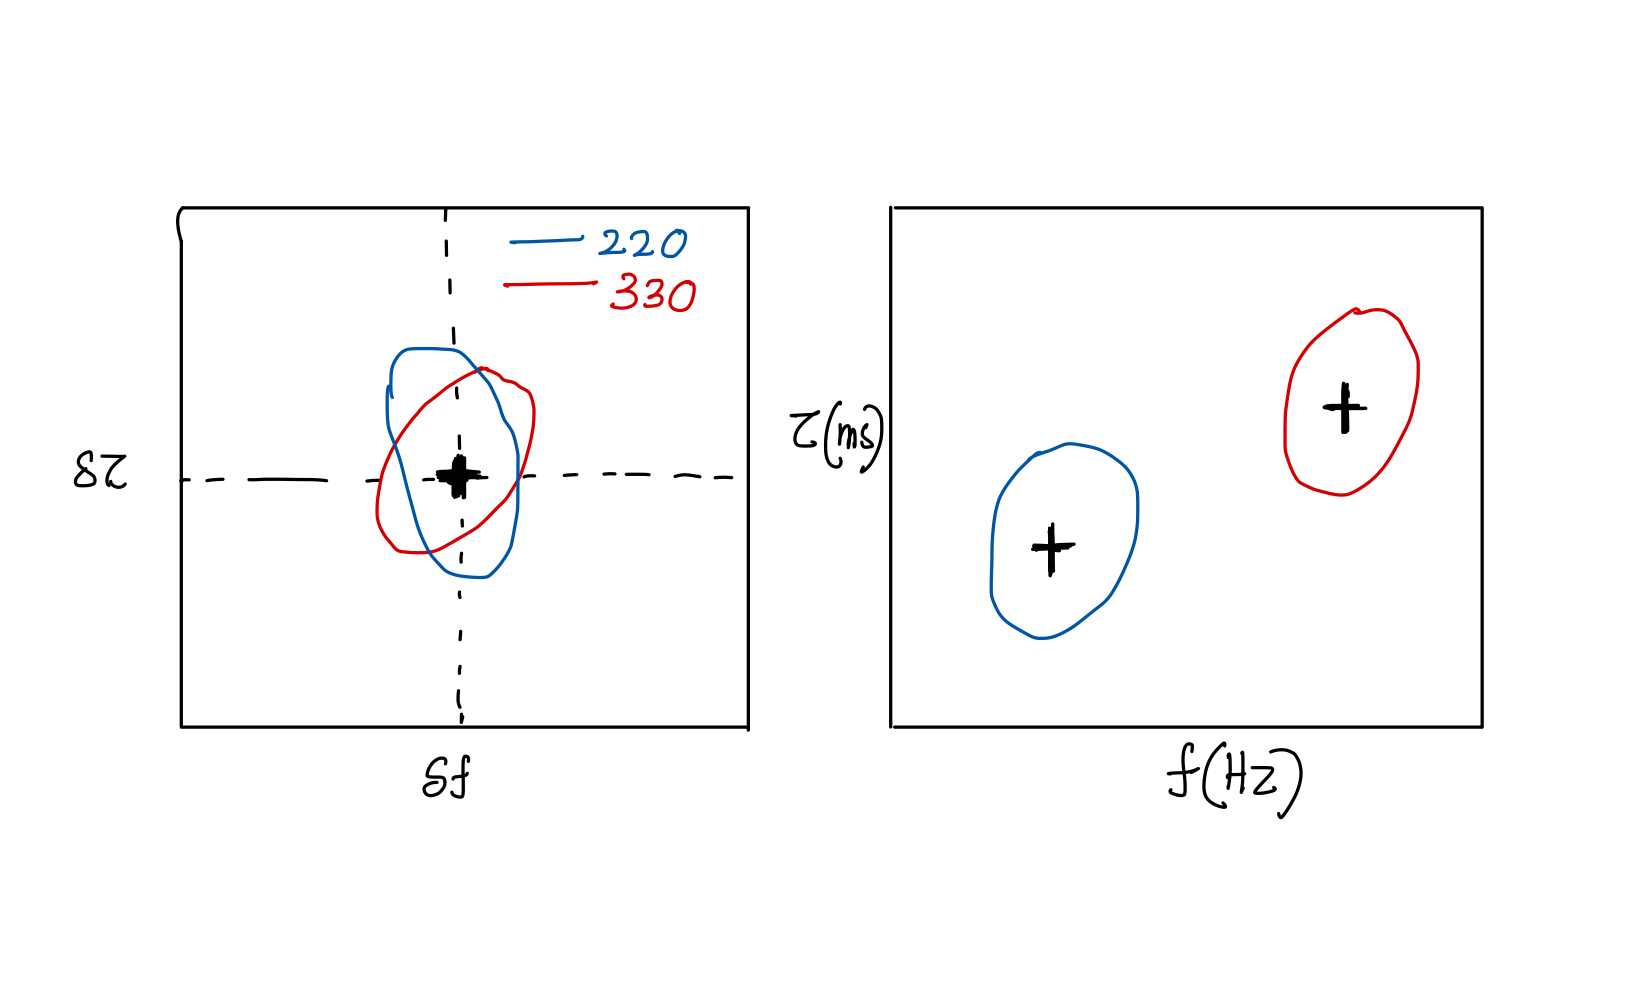
\includegraphics[width=0.5\textwidth]{figures/nohair_sxs_0166_placeholder.png}	
	\caption{\textcolor{red}{DEMO FIGURE; RUN ONGOING} Posterior probability distribution on the fractional deviations (left panel) and the reconstructed (right panel) frequency and damping time of the $(2,\pm 2)$ (blue curves) and $(3,\pm 3)$ (red curves) respectively, for a numerical relativity signal corresponding to a BBH merger of $q=6$,  $M=84 \Mo$ and SNR $75$. The plus signs mark the GR predictions.}
	\label{fig:nohair_sxs}
\end{figure}
%%%%%%%%%%%%%%%%%%%%%%%%%%%%%%%%%%%%%%%%%%%%%%%%%%%%%%%%%%%%%%%
%%%%%%%%%%%%%%%%%%%%%%%%%%%%%%%%%%%%%%%%%%%%%%%%%%%%%%%%%%%%%%%

\subsection{Results on actual LIGO-Virgo results}

The LIGO-Virgo Collaboration recently released their testing GR catalogue containing results of this test for all events observed during O3a ~\cite{Abbott:2020jks}, which passed a threshold for the total (source-frame) mass $\geq 50 \Mo$ and SNRs in the pre- and post-merger regions $\geq 8$.The pre- and post-merger regions of the signal are identified as the power in the frequency content of the signal before and after the signal reaches peak amplitude, as determined by the maximum likelihood parameter estimation template. For the purpose of \cite{Abbott:2020jks}, we used a mass threshold and restricted ourselves to the highest-mass events which were expected to be most promising to study merger-ringdown. However, since our method relies on doing a parameter estimation on the entire inspiral-merger-ringdown signal, we require the SNR to be beyond a certain threshold throughout the signal for reliable parameter estimation of the initial and final quantities. In fact the SNR threshold alone should be sufficient for the analysis, and for this paper we have relaxed the mass threshold. This has added two events, GW190630$\_$185205 and GW190828$\_$063405, to the list of events considered in \cite{Abbott:2020jks} \abhi{Runs ongoing and looking promising}. Fig.~\ref{fig:o1o2_events} shows results from these two events along with GW190519$\_$153544, GW190521$\_$074359, GW190910$\_$112807.

For the first time, in this paper, we present results on the relevant events from LIGO-Virgo's first and second observing runs, alongside the above events. Applying the same thresholds as above, we find three additional events which could be included in the analysis: GW150914, GW170104, GW170729. The other high-mass events from O1-O2, GW170809, GW170814, GW170818 and GW170823 do not have an SNR of $8$ in the merger-ringdown signal. For the three relevant signals, GW150914, GW170104 and GW170729, we provide the posterior distributions in $(\df{220}, \dtau{220})$ in Fig.~\ref{fig:o1o2_events}. We also reconstruct the effective QNM parameters, $(\fngr{220}, \taungr{220})$ which are tabulated in Table~\ref{tab:qnm_o1o2_results}. \footnote{See Table IV of \cite{Abbott:2020jks} for a list of the SNR thresholds. The paper quotes them for the purpose of the IMR consistency test, but the same thresholds have been used for the $pSEOB$ test as well.} Among all the GW signals detected so far, GW150914 (solid curve in Fig.~\ref{fig:o1o2_events})is unique in its loudness, mass as well as the clarity of the signal, leading to the first, and to date, best attempt in measuring the QNM frequencies CITE.

%%%%%%%%%%%%%%%%%%%%%%%%%%%%%%%%%%%%%%%%%%%%%%%%%%%%%%%%%%%%%%%
% O1-O2 events
%%%%%%%%%%%%%%%%%%%%%%%%%%%%%%%%%%%%%%%%%%%%%%%%%%%%%%%%%%%%%%%
\begin{figure}[h!]
	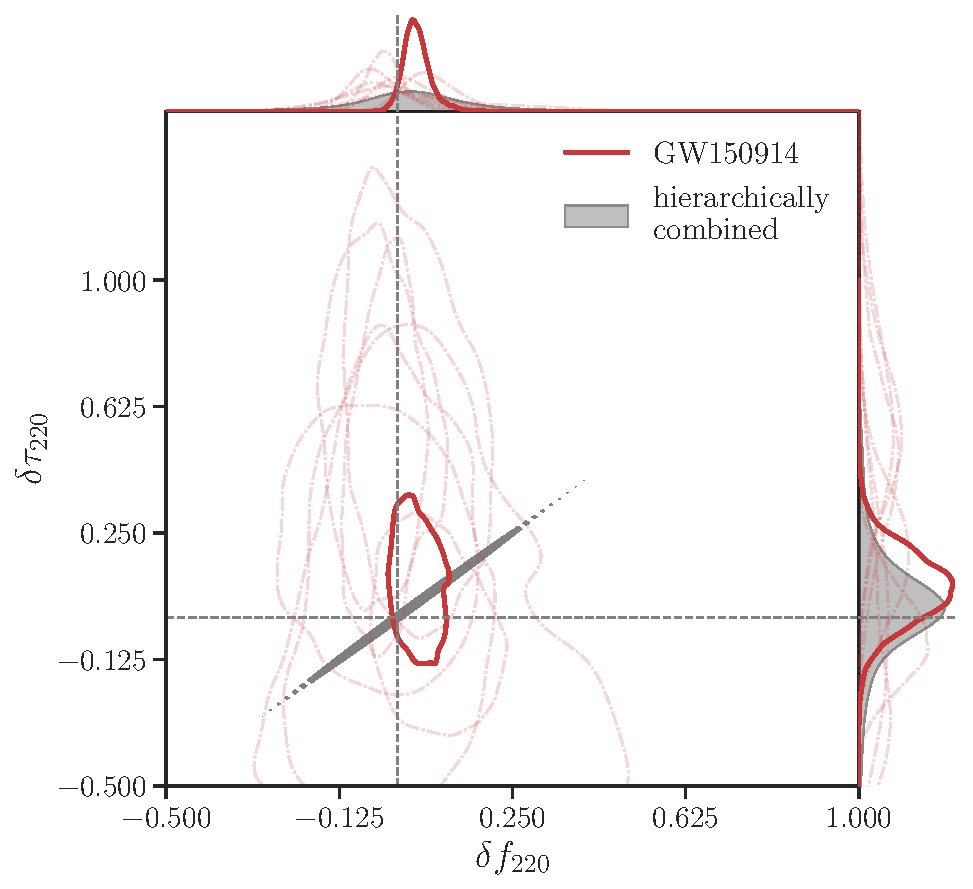
\includegraphics[width=0.5\textwidth]{figures/rin_pseob_results.pdf}
	\caption{\textcolor{red}{PRELIMINARY RESULT} The 90\% credible levels of the posterior probability distribution of the fractional deviations in the frequency and damping time of the $(2,\pm 2)$ QNM, $\{\df{220},\dtau{220}\}$ and their corresponding one-dimensional marginalized posterior distributions, for events from O1, O2 and O3a passing a SNR threshold of $8$ in both the pre- and post-merger signal. The solid red curve marks the constraint the best single-event constraint, GW150914, whereas the contraints from the other events are indicated by the dash-dot curves. The joint constraints on $\{\df{220},\dtau{220}\}$ obtained using multiplying the likelihoods from individual events is given by the filled grey contours.\abhi{add curves from joint likelihood}\abhi{add a hierarchical curve if we want to include that analysis}}
	\label{fig:o1o2_events}
\end{figure}
%%%%%%%%%%%%%%%%%%%%%%%%%%%%%%%%%%%%%%%%%%%%%%%%%%%%%%%%%%%%%%%
%%%%%%%%%%%%%%%%%%%%%%%%%%%%%%%%%%%%%%%%%%%%%%%%%%%%%%%%%%%%%%%

Finally, if we assume that the fractional deviations $(\df{220}, \dtau{220})$ take the same values in multiple events, we can assume the posterior of one event to be the prior for the next, and obtain a joint posterior probability distribution. For $N$ observations, where $P_j(\df{220}, \dtau{220} | d_j)$ is the posterior for the $j-th$ observation corresponding to the data set $d_j$, $j=1...N$, the joint posterior is given by:
\begin{equation}
P(\df{220}, \dtau{220} | \{d_j\}) = P(\df{220}, \dtau{220}) \prod _{j=1}^N \frac{P(\df{220}, \dtau{220} | d_j) }{P(\df{220}, \dtau{220})}
\end{equation}
where $P(\df{220}, \dtau{220})$ is the prior on $(\df{220}, \dtau{220})$. However, since we assume the prior on $(\df{220}, \dtau{220})$ to be flat or uniform, the joint posterior is equal to the joint likelihood.

We show these joint likelihoods on $(\df{220}, \dtau{220})$, as well as the corresponding one-dimensional marginalised distributions as filled grey curves in Fig.~\ref{fig:o1o2_events}. These are the strongest constraints on possible deviations in the measurement of $(\df{220}, \dtau{220})$ to date using our method. \abhi{perhaps show 2 joint posteriors: only O3a and O3a+O1-O2 to explicitly show the tightening of the joint constraints by adding the O1-O2 events} \abhi{add text on the hierarchical analysis if we want to include that analysis}

\begin{table}
\begin{flushleft}
\begin{tabular}{llllllll}
\toprule
Event & \multicolumn{2}{c}{Redshifted} & \hphantom{X} & \multicolumn{2}{c}{Redshifted} \\
& \multicolumn{2}{c}{frequency [Hz]} & \hphantom{X} & \multicolumn{2}{c}{damping time [ms]} \\[0.075cm]
\hline
& IMR  & pSEOB & \hphantom{X} & IMR  & pSEOB \\
\hline

GW150914 &
$249^{+9}_{-7}$ &
$-$ &
\hphantom{X} &
$4.1^{+0.3}_{-0.2}$ &
$-$
\\[0.075cm]

GW170104 &
$286^{+16}_{-27}$ &
$-$ &
\hphantom{X} &
$3.5^{+0.4}_{-0.3}$ &
$-$
\\[0.075cm]

GW170729 &
$161^{+13}_{-14}$ &
$-$ &
\hphantom{X} &
$7.8^{+1.8}_{-1.5}$ &
$-$
\\[0.075cm]

GWGW190630$\_$185205 &
$-$ &
$-$ &
\hphantom{X} &
$-$ &
$-$
\\[0.075cm]

GW190828$\_$063405,170729 &
$-$ &
$-$ &
\hphantom{X} &
$-$ &
$-$
\\[0.075cm]
\hline
\bottomrule
\end{tabular}
\caption{\textcolor{red}{NOT COMPLETE}}
\label{tab:qnm_o1o2_results}
\end{flushleft}
\end{table}

\section{Discussion}\label{sec:discussion}

\section*{ACKNOWLEDGEMENTS}\label{sec:acknowledgements}
LIGO Clusters


\iffalse
\abhi{A comparison with pyRING}
\abhi{damped sinusoid results}
\fi

\pagebreak

\appendix
\section{Study of syetematics on ringdown measurements}\label{sec:noise_systematics}

\iffalse
\abhi{A small summary of the noise systematics study that was done for S190521g to show that the deviations seen were consistent with systematics due to noise. The study include 2 separate sections: in Gaussian noise, and in real LIGO-Virgo noise immediately adjacent to the actual event.}
\fi

In Section~\ref{sec:method}, we mentioned that the expression of the Bayesian likelihood function outlined in Eqs.~\ref{eq:likelihood} and \ref{eq:nwip} is only valid if the interferometric noise can be described as a stationary Gaussian process. LIGO-Virgo noise, however, frequently has non-stationary and/or non-Gaussian features, for example glitches, which can affect parameter inferences unless appropriately accounted for. Here we demonstrate with an example of a GW190521-like simulated signal, systematic biases likely originating from an incomplete understanding of the noise. 

%%%%%%%%%%%%%%%%%%%%%%%%%%%%%%%%%%%%%%%%%%%%%%%%%%%%%%%%%%%%%%%
%%%%%%%%%%%%%%%%%%%%%%%%%%%%%%%%%%%%%%%%%%%%%%%%%%%%%%%%%%%%%%%
\begin{figure}
	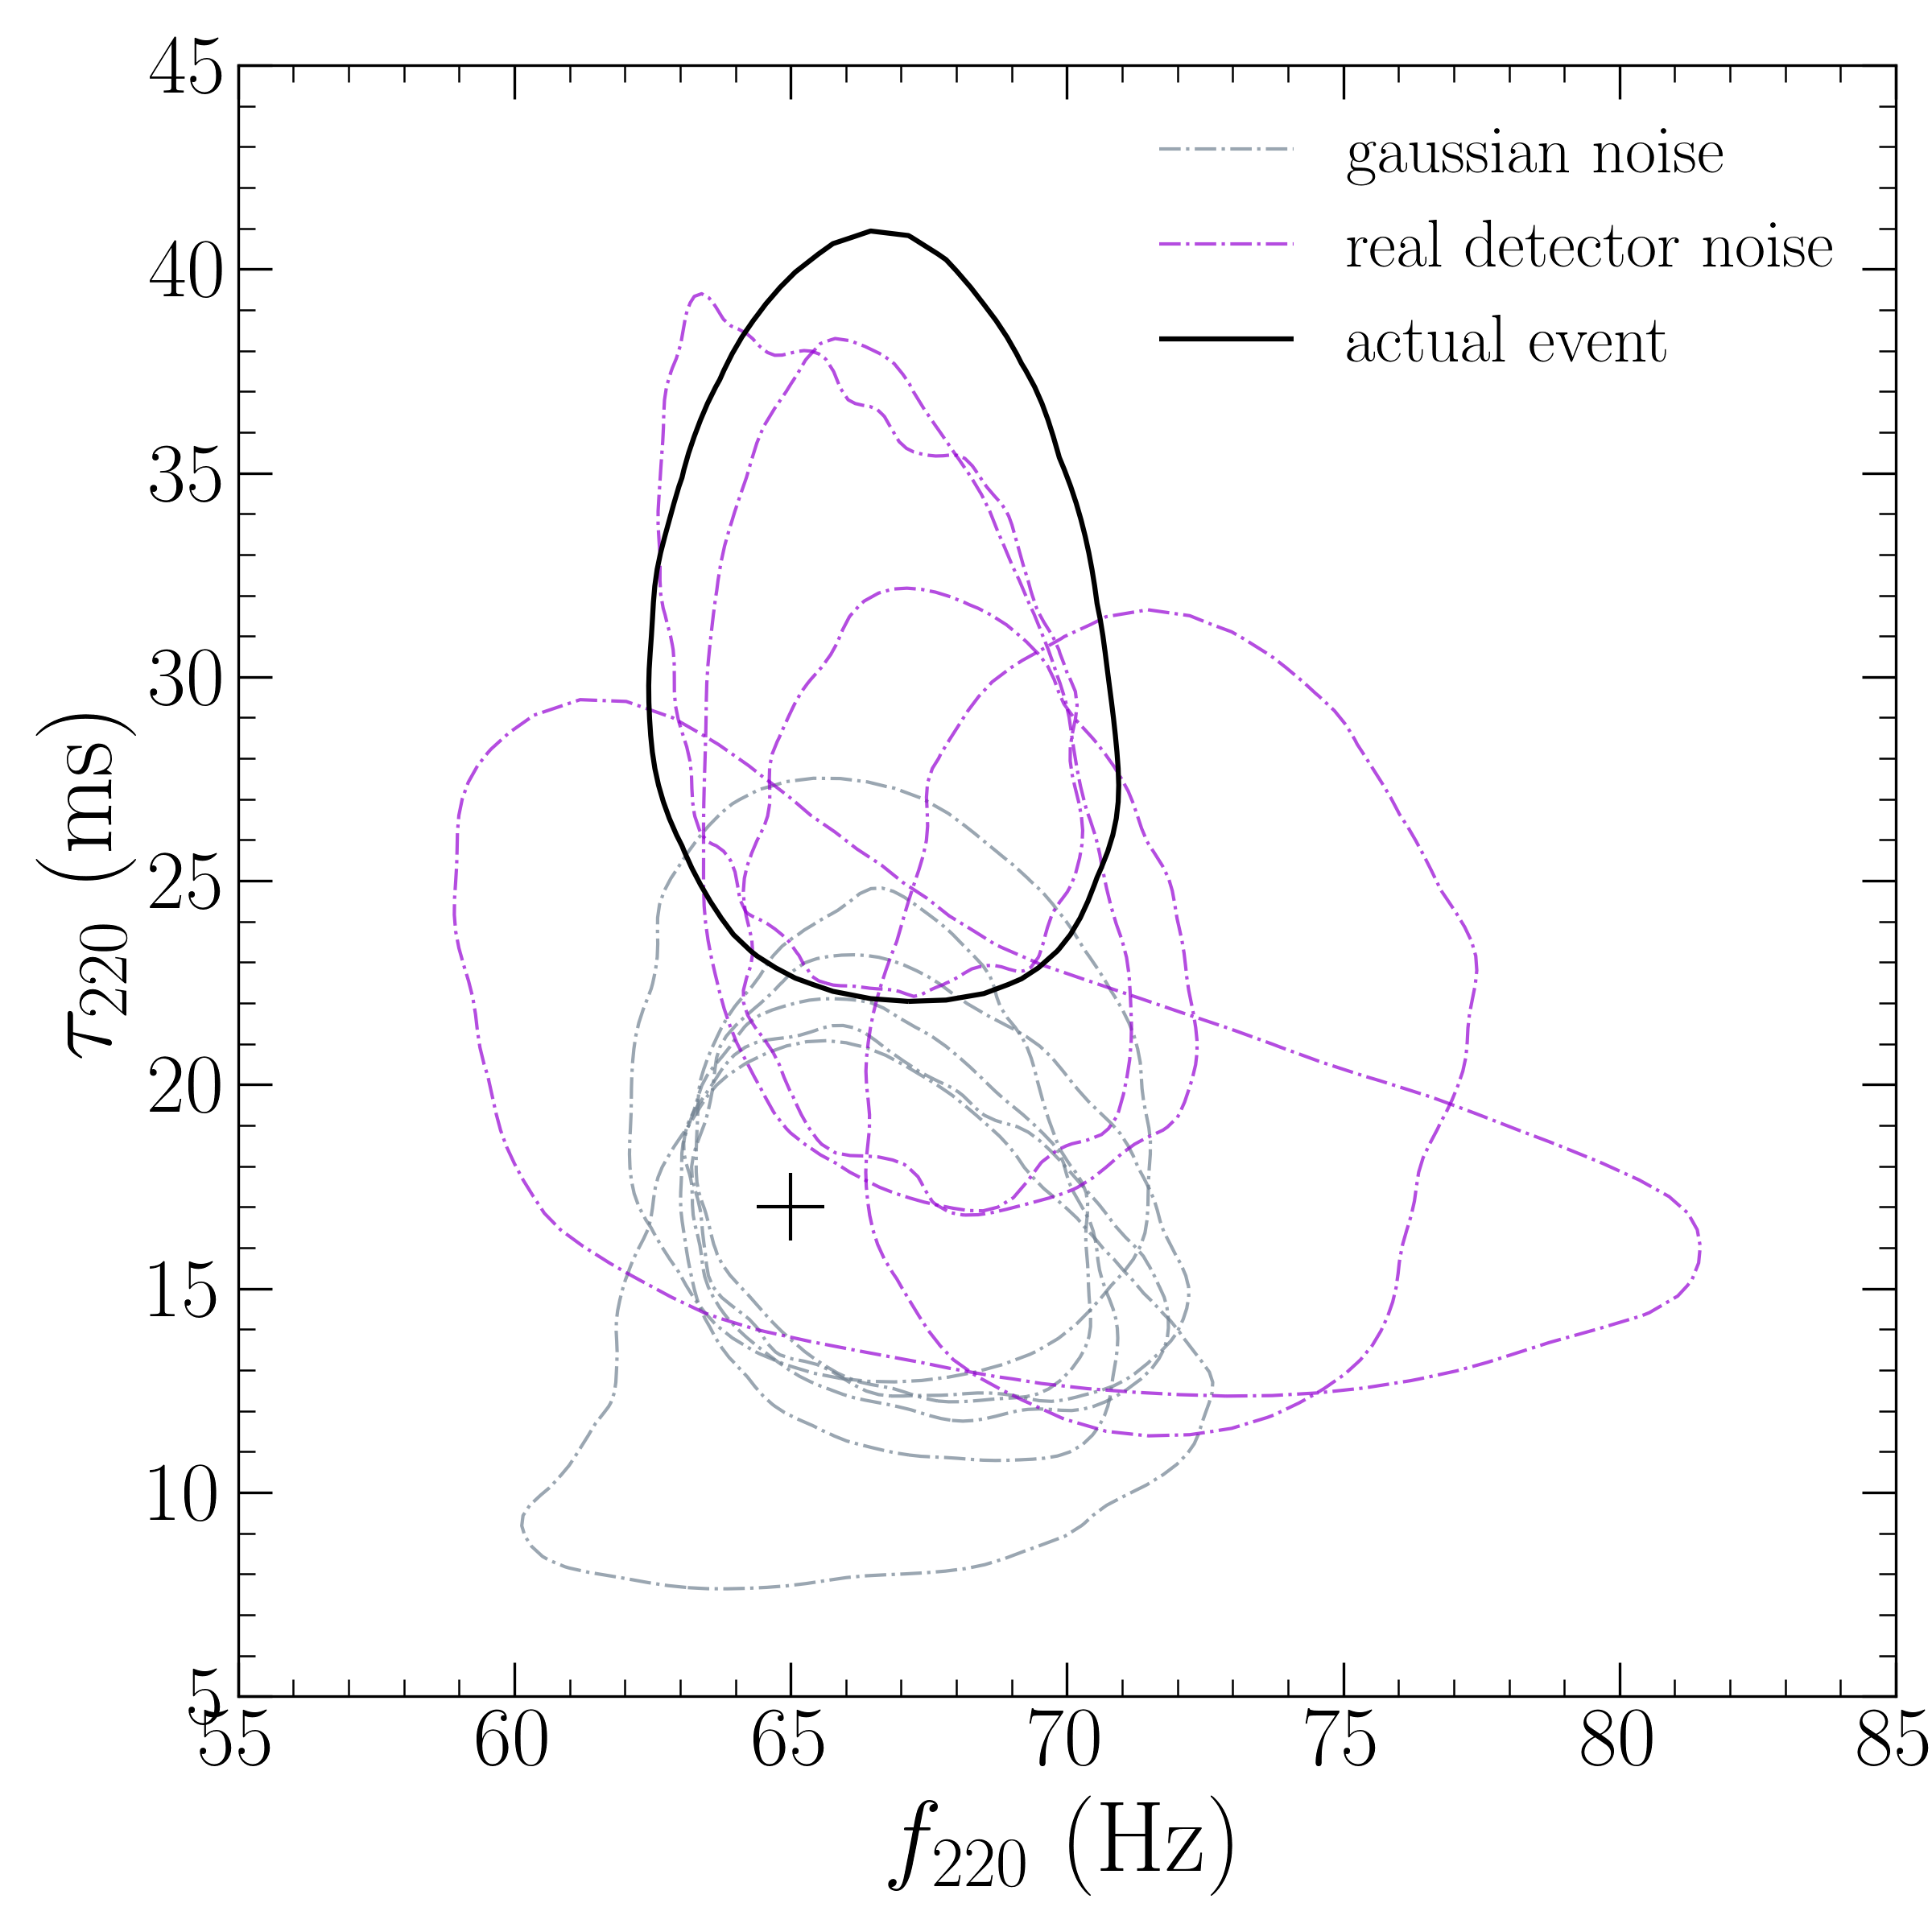
\includegraphics[width=0.5\textwidth]{figures/S190521g_swinjs.png}
	\caption{\textcolor{red}{FINAL RESULT} 90 \% credible level on the posterior probability distribution of the frequency and damping time of $(2,\pm 2)$ mode, $(\fgr{220}, \taugr{220}$ from simulations of an \texttt{NRSur7dq4} GW signal with parameters similar to the GW event, GW190521, in Gaussian noise (grey dot-dashed lines) and real interferometric noise (pink dot dashed lines). The GR prediction for the frequency and damping time is indicated by the black cross. While the Gaussian noise simulations are consistent with the prediction, at least 3 or the 5 real noise simulation are not. For comparison, we also plot the 90 \% credible level for the actual event, GW190521.}
	\label{fig:21g_systematics}
\end{figure}
%%%%%%%%%%%%%%%%%%%%%%%%%%%%%%%%%%%%%%%%%%%%%%%%%%%%%%%%%%%%%%%
%%%%%%%%%%%%%%%%%%%%%%%%%%%%%%%%%%%%%%%%%%%%%%%%%%%%%%%%%%%%%%%

We use as our underlying GR signal, an NR waveform (using the waveform model \texttt{NRSur7dq4}) with parameters similar to the actual event GW190521 (as reported in Table I of \cite{Abbott:2020tfl}). The predictions of the frequency and damping time for the GR signal we choose are indicated by the black cross in Fig.~\ref{fig:21g_systematics}, and for comparison, the results on the actual signal are shown with a black solid curve. It would appear that while the measurement of the frequency is consistent with the prediction, we overestimate the damping time. 

The underlying NR signal is expected to be precessing, and since the $pSEOB$ model is built on an aligned-spin GR model, a lack of precession could bias measurements. We explore effects of possible waveform systematics by injecting the signal is coloured Gaussian noise. In this case, since the understanding of the noise realisations is complete, any measurement biases could only arise from incomplete understanding of the underlying signal. We find (grey curves in Fig.\ref{fig:21g_systematics}) our results to be consistent with the prediction thus ruling out a lack of precession to be a likely cause for the bias in the damping time measurement of the actual signal.

We subsequently study the effects of possible noise systematics by injecting the same \texttt{NRSur7dq4} GW signal in different realisations of actual interferometric noise around the real event GW190521. Since the PSDs of the GW detectors are expected to vary over longer durations of time, we select 5 different noise realisations over a segment of 2.5 hours of coincident data in both the LIGO detectors centred at the time of the actual event. The noise properties in this chunk of data, and consequently for all 5 simulated signals, is expected to be the closest to that for the actual event. The results are indicated by pink curves in Fig.~\ref{fig:21g_systematics}. For 3 of the 5 noise realisations, corresponding to $t_0-1$ hour, $t_0+0.5$ hours, and $t_0+1$ hour we recover a damping time similar to the actual event, where $t_0$ is the GPS time of the actual event. For the other two noise realisations, we estimate the consistent damping time but an off-set frequency, while the fifth noise realisation is consistent with both predictions. The SNR in the L1 Livingston detector goes down by more than 3 in some runs, indicative of how a variation in the noise strongly affects our ability to infer parameters. This also seems to indicate that a bias in the measurements of the damping time for the actual event can be unaccounted noise systematics.

\section{Correlations between GR and non-GR parameters}\label{sec:correlations}
\abhi{Do we want a separate appendix to discuss Fig.~\ref{fig:gr_ngr_comparison}? Or is the reference in the main text currently, sufficient?}

%%%%%%%%%%%%%%%%%%%%%%%%%%%%%%%%%%%%%%%%%%%%%%%%%%%%%%%%%%%%%%%
% modified GR signal: GR vs nonGR recovery comparison
%%%%%%%%%%%%%%%%%%%%%%%%%%%%%%%%%%%%%%%%%%%%%%%%%%%%%%%%%%%%%%%
\begin{figure*}[h!]
	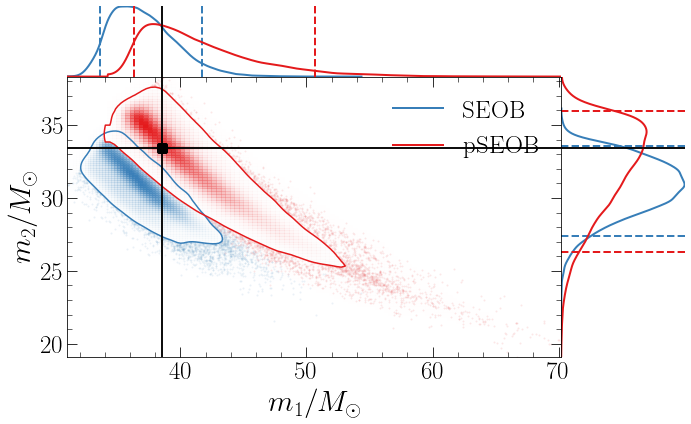
\includegraphics[width=0.5\textwidth]{figures/GW150914_simulated_signal_0p5_gr_ngr_m1m2.png}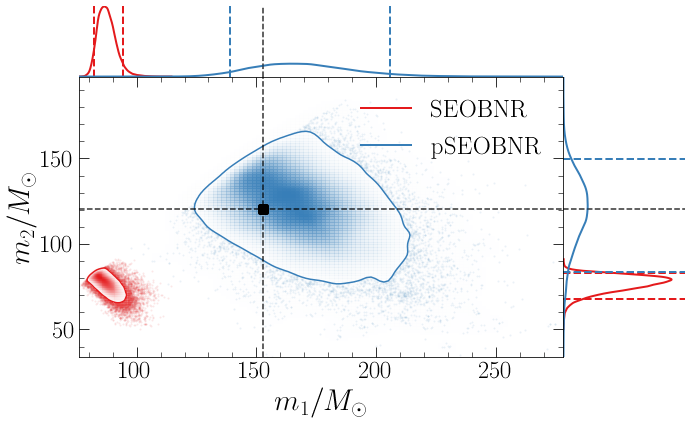
\includegraphics[width=0.5\textwidth]{figures/GW190521_simulated_signal_0p5_gr_ngr_m1m2.png}
	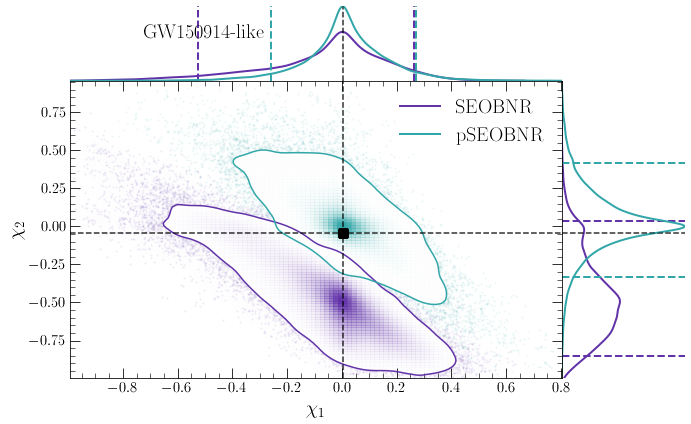
\includegraphics[width=0.5\textwidth]{figures/GW150914_simulated_signal_0p5_gr_ngr_a1za2z.png}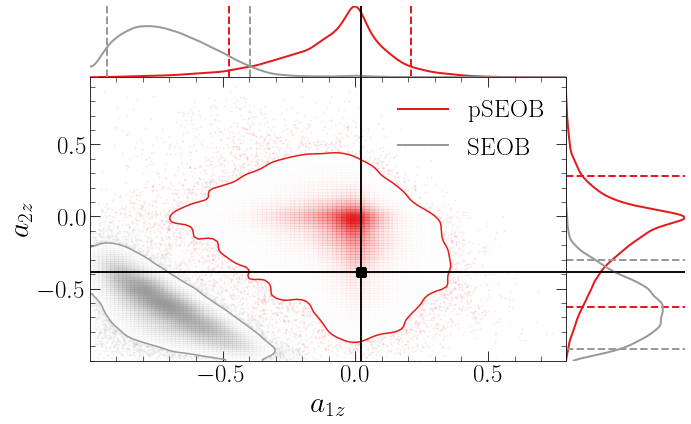
\includegraphics[width=0.5\textwidth]{figures/GW190521_simulated_signal_0p5_gr_ngr_a1za2z.png}	
	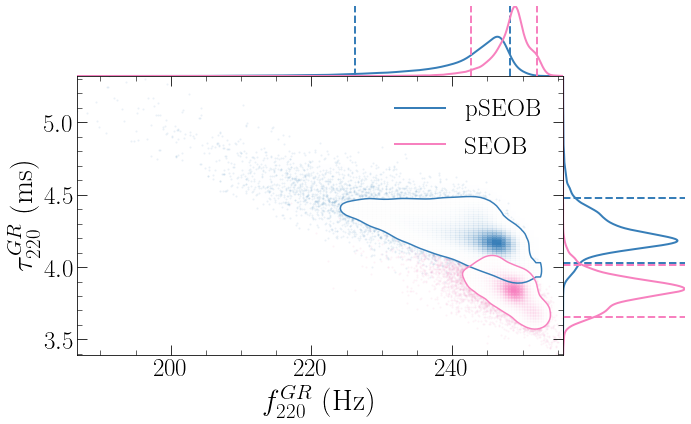
\includegraphics[width=0.5\textwidth]{figures/GW150914_simulated_signal_0p5_gr_ngr_fgrtaugr.png}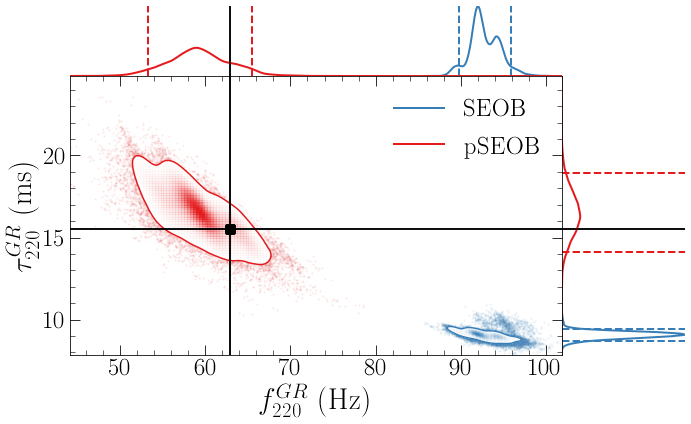
\includegraphics[width=0.5\textwidth]{figures/GW190521_simulated_signal_0p5_gr_ngr_fgrtaugr.png}
	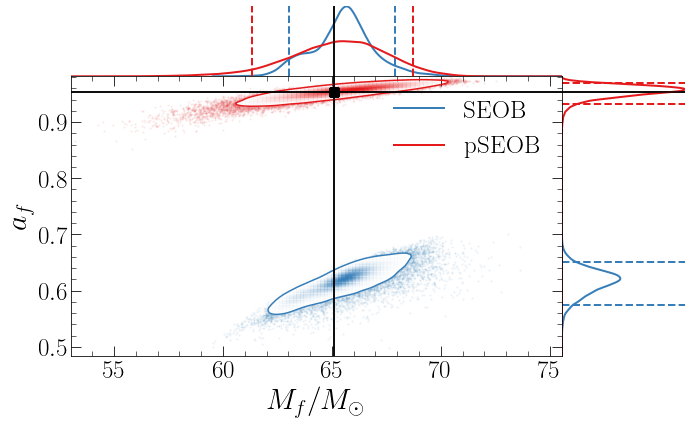
\includegraphics[width=0.5\textwidth]{figures/GW150914_simulated_signal_0p5_gr_ngr_Mfaf.png}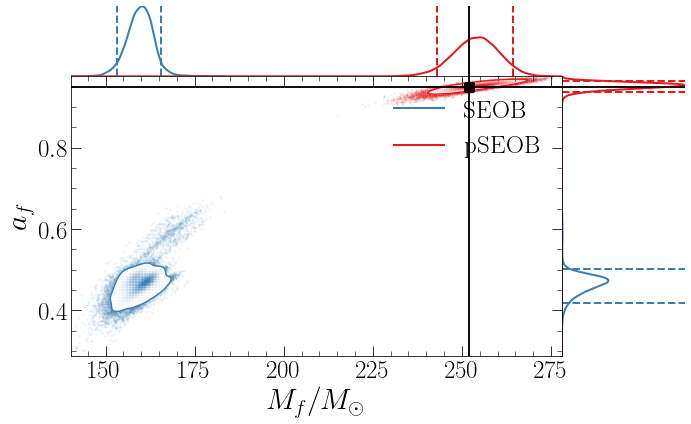
\includegraphics[width=0.5\textwidth]{figures/GW190521_simulated_signal_0p5_gr_ngr_Mfaf.png}
	\caption{\textcolor{red}{FINAL RESULT} Comparison of the recovered parameters when the underlying signal is assumed to be a GR signal or a modified GR signal. In both cases, the actual underlying signal is a modified GR signal with parameters similar to GW150914 (left panels) and GW190521 (right panels) respectively. The initial parameters are given in Table~\ref{tab:injection_values}, with the QNM parameters defined by $\df{220} = \dtau{220} = 0.5$. For the GW150914 (GW190521) contours, the $SEOB$ and $pSEOB$ recoveries are indicated by blue (red) and pink (grey) curves respectively. The panels (from top to bottom) show the recoveries in (detector-frame) initial masses (first row), z-components of dimensionless initial spins (second row), GR predictions of frequency and damping time (third row) and the remnant mass and spin predictions ($M_f, a_f$) from the frequency and damping time (obtained by inverting the Berti fits) CITE}
	\label{fig:gr_ngr_comparison}
\end{figure*}
%%%%%%%%%%%%%%%%%%%%%%%%%%%%%%%%%%%%%%%%%%%%%%%%%%%%%%%%%%%%%%%
%%%%%%%%%%%%%%%%%%%%%%%%%%%%%%%%%%%%%%%%%%%%%%%%%%%%%%%%%%%%%%%


%
\bibliographystyle{apsrev}
\bibliography{intro_paper}

\end{document}